\documentclass[12pt]{article}
\setlength\parindent{0pt}
\usepackage{fullpage}
\usepackage{amsmath}
\usepackage{lscape}
\usepackage[table,xcdraw]{xcolor}
\usepackage{graphicx}
\usepackage[margin=0.5in]{geometry}
\setlength{\parskip}{4mm}
\def\LL{\left\langle}   % left angle bracket
\def\RR{\right\rangle}  % right angle bracket
\def\LP{\left(}         % left parenthesis
\def\RP{\right)}        % right parenthesis
\def\LB{\left\{}        % left curly bracket
\def\RB{\right\}}       % right curly bracket
\def\PAR#1#2{ {{\partial #1}\over{\partial #2}} }
\def\PARTWO#1#2{ {{\partial^2 #1}\over{\partial #2}^2} }
\def\PARTWOMIX#1#2#3{ {{\partial^2 #1}\over{\partial #2 \partial #3}} }
\newcommand{\BI}{\begin{itemize}}
\newcommand{\EI}{\end{itemize}}
\newcommand{\BE}{\begin{displaymath}}
\newcommand{\EE}{\end{displaymath}}
\newcommand{\BNE}{\begin{equation}}
\newcommand{\ENE}{\end{equation}}
\newcommand{\BEA}{\begin{eqnarray}}
\newcommand{\EEA}{\nonumber\end{eqnarray}}
\newcommand{\EL}{\nonumber\\}
\newcommand{\la}[1]{\label{#1}}
\newcommand{\ie}{{\em i.e.\ }}
\newcommand{\eg}{{\em e.\,g.\ }}
\newcommand{\cf}{cf.\ }
\newcommand{\etc}{etc.\ }
\newcommand{\Tr}{{\rm tr}}
\newcommand{\etal}{{\it et al.}}
\newcommand{\OL}[1]{\overline{#1}\ } % overline
\newcommand{\OLL}[1]{\overline{\overline{#1}}\ } % double overline
\newcommand{\OON}{\frac{1}{N}} % "one over N"
\newcommand{\OOX}[1]{\frac{1}{#1}} % "one over X"

\pagenumbering{gobble}

\begin{document}

%\begin{center}
%	\Large Exercise 1: on combining rotation and translation
%\end{center}
%
%\begin{minipage}{0.6\textwidth}
%A Yo-Yo consists of a cylinder of radius $R$ with a thin slit cut in it. Inside the slit is a smaller inner cylinder of radius $r$ with a string attached to it and then wound around the cylinder. Note that the moment of inertia of a cylinder of radius $R$ is $I=\frac{1}{2}mR^2$; since the slit in the Yo-Yo is so thin, you do not need to consider it in computing the moment of inertia. (Thus, both have the same moment of inertia: $I=\frac{1}{2}mR^2$.)
%
%If a person holds the end of the string and drops the Yo-Yo, it will begin to spin as it falls, unwinding the string as it does. 
%
%\bigskip\bigskip
%
%a) Suppose that you have a red Yo-Yo with $r=0.1 R$ (that is, with a very small inner cylinder) and a blue Yo-Yo with $r=0.4 R$ (with a thicker inner cylinder). Predict which one will fall faster when it is dropped, and describe why it will do so. \textit{(You shouldn't do any calculations here.)}
%\end{minipage}
%\begin{minipage}{0.20\textwidth}
%	\begin{center}
%	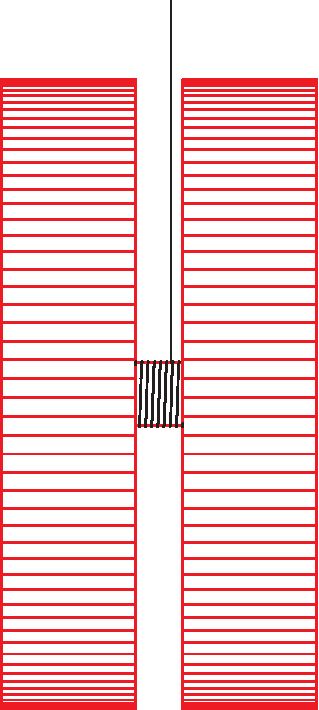
\includegraphics[width=0.7\textwidth]{red-crop.pdf}
%	\end{center}
%\end{minipage}
%\begin{minipage}{0.20\textwidth}
%		\begin{center}
%	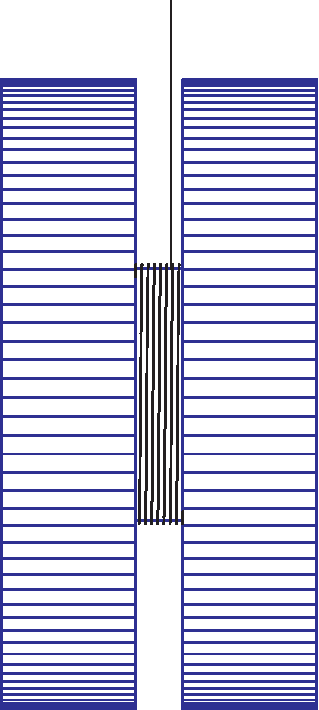
\includegraphics[width=0.7\textwidth]{blue-crop.pdf}
%		\end{center}
%\end{minipage}
%
%
%\vspace{1.5in}
%
%b) Now, you'll calculate the downward acceleration of the Yo-Yo. In this case, the Yo-Yo both {\it translates} and {\it rotates} as it does so
%
%Start by drawing an extended force diagram for the Yo-Yo, showing all the forces acting on it {\it and where they act}.
%
%\vspace{2in}
%
%\newpage
%
%c) Since it both translates and rotates, you will need both $\vec F = m \vec a$ to relate the forces on it to its translational acceleration and $\tau = I \alpha$ to relate the torques on it to its linear acceleration. Construct both of these equations, using the forces that appear on your force diagram. \textit{(Hint: The tension in the string both applies a torque to the Yo-Yo and affects its translational acceleration.)}
%
%\vspace{2.5in}
%
%d) In the above two equations, you will have three unknowns: the tension in the string, the translational acceleration, and the angular acceleration $\alpha$. However, you can relate two of them to each other. What is that relation? \textit{(Hint: Think carefully about minus signs here!)}
%
%\vspace{1in}
%
%e) Now you should have enough information to solve for $a$ in terms of $g$, $r$, and $R$. Once you have a value for your acceleration, call your GTA or coach over and have them check your work. Discuss with them whether the red or blue Yo-Yo in part (a) would fall faster. 
%
%\newpage
%
%\begin{center}
%	\Large Exercise 2
%\end{center}
%
%Consider the demonstration you saw in class yesterday. A person stands on top of a platform that is free to rotate.
%
%a) Estimate the moment of inertia of the person around their center. You will need to figure out which of our simple shapes best approximates a person, then estimate the person's radius and mass. \textit{(The table of moments of inertia is at the end.)}
%
%\vspace{1in}
%
%b) Someone else standing on the ground carries a bicycle wheel filled with concrete of mass $m=5$ kg with radius 30 cm. They make the bicycle wheel spin at an angular velocity $\omega = 20$ radians/sec, turn it so that it is spinning clockwise when viewed from above, then hand it to the person standing on the platform. 
%
%When the person standing on the platform grabbed the wheel to stop it from spinning, they began to rotate slowly. Determine which direction and how fast they begin to rotate after they do this.
%
%\vspace{3in}
%\newpage
%
%c) Imagine now that instead of grabbing the wheel, they turned it upside down, so it would be spinning counterclockwise rather than clockwise when seen from above. Without doing any mathematics, predict what should happen. Call your TA or coach over to discuss with your group.
%
%\vspace{2in}
%
%d) Now, calculate which direction they will rotate and how fast when they rotate the wheel upside down. Does the result of your calculation agree with your prediction?
%\vfill
%
%\begin{center}
%	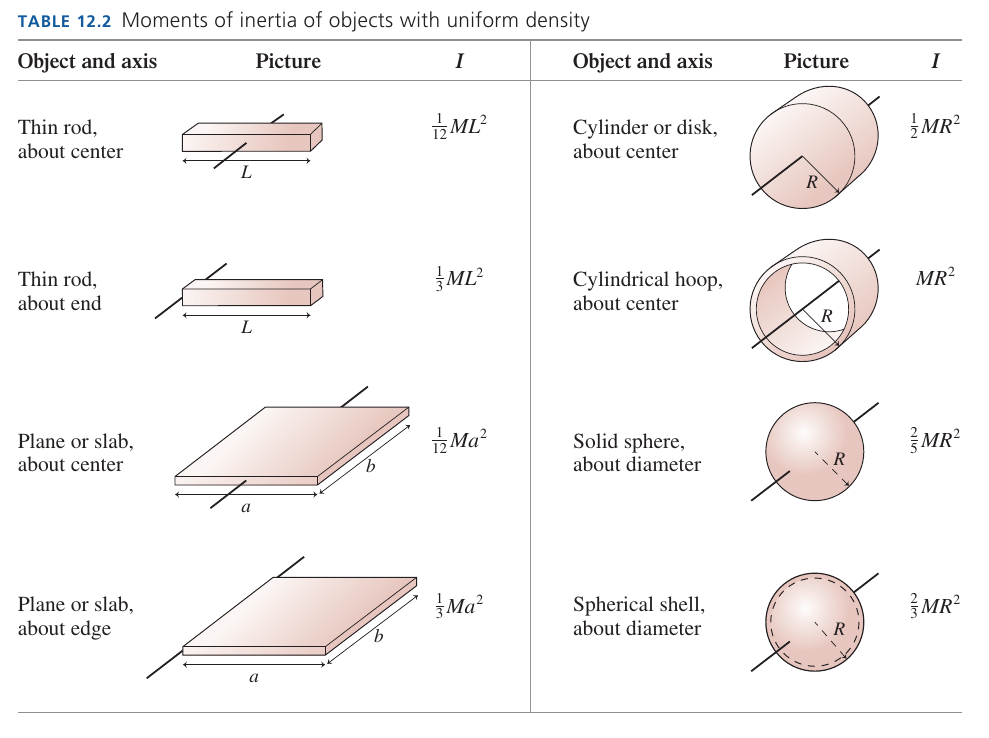
\includegraphics[width=4in]{moment-table.png}
%\end{center}
%
%\newpage
%
%% A bucket of mass $m$ hangs from a string wound around a pulley 
%%(a solid cylinder) with mass $M$ and radius $r$. When the bucket is
%%released, it falls, unwinding the string.
%%
%%\begin{enumerate}
%%
%%\item Draw force diagrams for the bucket and the pulley. Note that since the pulley rotates, you will need
%%to draw an extended force diagram for it, drawing the object and labeling where each force acts.
%%
%%\vspace{3in}
%%
%%\item In terms of the forces in your force diagrams, write an expression for the net torque on the pulley.
%%
%%\vspace{1in}
%%
%%\item Write down Newton's laws of motion -- $\sum \vec F = m \vec a$ for translation, and $\sum \tau = I \alpha$
%%-- for each object. (One object moves, and the other turns...)
%%
%%\vspace{2in}
%%
%%
%%\newpage
%%
%%\item What is the relationship between the angular acceleration $\alpha$ of the pulley and the linear acceleration
%%$a$ of the bucket? (The answer may be different depending on how you have drawn your pictures and your choice of
%%coordinate system.)
%%
%%\vspace{1in}
%%
%%\item Calculate the acceleration of the bucket in terms of $m$ and $M$.
%%
%%\vspace{4in}
%%
%%\item Suppose that the pulley were a hollow cylinder with the same mass. How would this acceleration change?
%
%%\newpage
%%\end{enumerate}
%
%%A simplified model of a car or truck can be thought of as shown below. Consider
%%the body of the vehicle to be a uniform plate of mass $M$, supported by the
%%normal force of two axles, each located a distance $L/6$ from each end.
%%The engine, also of mass $M$, is located a distance $L/6$ from the front. (Don't worry about 
%%distinguishing the left wheels from the right ones; you can treat ``front wheels'' and ``back wheels''
%%as single forces.) Note that the car is pointed to the left here (since the engine is in the front).
%%
%%Some terminology, for those who are not familiar:
%%
%%\BI
%%\item ``Front wheel drive'' means that the engine is coupled only to the front wheels, and is only able to use 
%%them to provide forward traction. This means that the maximum traction is $\mu_s F_{N, \rm front}$.
%%\item ``Rear wheel drive'' means that the engine is coupled only to the back wheels, and is only able to use 
%%them to provide forward traction. This means that the maximum traction is $\mu_s F_{N, \rm back}$.
%%\item ``All-wheel drive'' or ``four-wheel drive'' mean that the engine is coupled to both sets of wheels,
%%and may use the static friction of both of them to provide traction.
%%\EI
%%
%%\begin{center}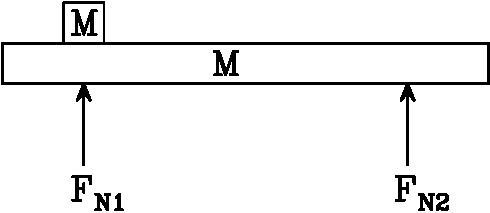
\includegraphics[width=0.5\textwidth]{car-crop.pdf}\end{center}
%%\begin{enumerate}
%%
%%\item Without doing any mathematics, do you expect the normal force from the front wheels 
%%or from the rear wheels to be larger? Why?
%%
%%\vspace{1in}
%%
%%\item Draw an extended force diagram for the vehicle.
%%
%%\newpage
%%
%%\item Calculate the normal forces $F_{N1}$ and $F_{N2}$ exerted by each axle.
%%
%%\vspace{3in}
%%
%%\item Suppose that the coefficient of friction between the wheels and the ground is $\mu_s$. What is the maximum
%%traction force that the car can apply if it is front wheel drive? (Most small cars
%%are front wheel drive.)
%%
%%\vspace{3.5in}
%%
%%\item What is the maximum traction force that the vehicle can apply if it is rear wheel drive? (Most trucks are rear
%%wheel drive.)
%%
%%\vspace{3.5in}
%%
%%\item Often people with two-wheel-drive pickup trucks will pile snow in the back of the truck during the Syracuse winter.
%%Why do they do this?
%%
%%As a hint, the thing that determines whether you will get stuck or not in slippery conditions is often the ratio between the traction force and the total mass of the vehicle.
%
%
%\newpage
%
%\newpage


\Large
\centerline{\sc{Recitation Exercises}}
\normalsize
\centerline{\sc{29 April}}

In this exercise of the semester, you will study {\it transmissions} -- the assemblages of gears that transmit torque from a motor to the machine that it turns. For instance, the motor might be the engine of a car or the legs of a cyclist; the ``machine'' is the drive wheel applying traction to the ground. This works the same for all sorts of machines that use rotary motion to transmit power.

This exercise is a little different than others: it is designed to let you explore a very useful sort of device we see around us. If your group completes this exercise fully, you will earn five points extra credit. We intend for you to work actively with your coaches and TA's here, so ask us questions!

In all of these cases, the motor applies a torque to the driveshaft, which is connected to a machine that applies an equal and opposite torque. Thus, the motor delivers power to the machine. For this problem, the motor will always be spinning at a constant angular velocity, so $\sum \tau = 0$.

Motors have two limitations: 

\begin{itemize}
	\item They are limited in the torque that they can apply. For instance, for a human riding a bicycle, there is only so much force they can apply to the pedals.
	\item They are limited in their angular velocity. For instance, a person riding a bicycle can only spin their legs so fast.
\end{itemize}

We will see how we can partially overcome these limitations using gears. Let's think about this in an idealized case of an electric motor spinning a machine, and then apply it to a person riding a bike. Suppose that the motor can apply a maximum torque $\tau_{\rm {max}}=100~\rm N \cdot \rm m$ to the driveshaft, but it has a maximum angular velocity $\omega_{\rm max} = 50$ rad/sec.

Let's imagine a situation where the motor is always applying maximum torque, and see what happens to the machine the motor is driving.

\bigskip

\begin{enumerate}

\item What is the maximum power that the motor can deliver to the machine? \textit{(Hint: For translational motion, $P = \vec F \cdot \vec v$. What is the analogous formula for rotation?)} 

Fill in the first row of the table on the back; note that since the motor and machine are connected directly, the torque and angular velocity of the motor are the same as those of the machine.
	
	
	\vspace{0.8in}
\item However, in general, machines need to run at different speeds; for instance, cars can drive at many different speeds. Suppose that the operator of the machine wants to run it at low speed -- say, at 25 rad/s. Can the motor still deliver the same power in this case? If not, how much power can it deliver? Complete the second row of the table on the back.
	
\vspace{1.5in}
\newpage



 The motor is simply {\it unable} to rotate any faster than 50 rad/sec. For instance, running the machine at $\omega = 100$ rad/s is impossible with the motor alone. Since the machine operator may want to run the machine at any speed, and will likely want the most power from the motor at {\it any} speed, they construct a transmission out of gears.
\medskip

\begin{minipage}{0.4\textwidth}
	
	In this figure, the motor is connected to the red gear with $r_{in}=10$ cm; the machine is connected to the blue gear. We will first think about how this transmission works using
	a single blue gear with a radius of $R_{out}=20$~cm in order to understand the principles at work here; then, we will think about the advantages of {\it shifting} gears,
	as in a bicycle or car transmission.
	
\end{minipage}
\begin{minipage}{0.49\textwidth}
	\begin{center}
		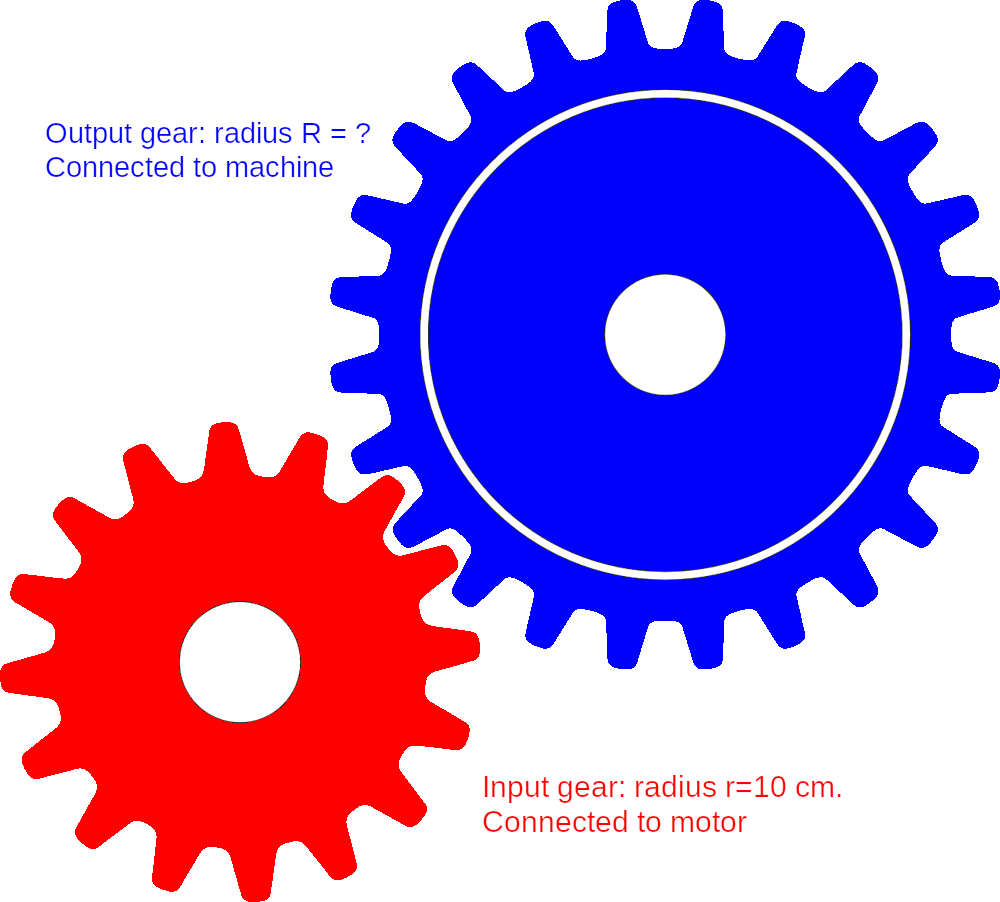
\includegraphics[width=0.8\textwidth]{Gears.png}
	\end{center}
\end{minipage}
\medskip

Here everything is rotating at a constant angular velocity. This means that the motor applies a clockwise torque to the red gear; the blue gear applies an equal and opposite counterclockwise torque to it.

\item Newton's third law applies to the forces that the two gears exert on each other: the two gears push on each other with equal and opposite forces. Given this, determine the relationship between $\tau_{\rm {motor}}$ (the torque the motor applies to the red gear) and $\tau_{\rm {machine}}$ (the torque the blue gear applies to the machine) in terms of $r_{in}$ and $R_{out}$. Record this formula on the back page. Note that the ratio between $r_{in}$ and $R_{out}$ appears in this formula: this is called the {\it gear ratio}, and is critically important.

\vspace{1.8in}

\item The velocities of the gears' teeth must also be the same as they turn. Given this, determine the relationship between $\omega_{\rm {motor}}$ (the speed at which the motor and red gear turn) and $\omega_{\rm {machine}}$ (the speed at which the blue gear and the machine turn). Again, you should have a result that depends on the gear ratio. Record this formula on the back page; call your coach or TA over to check your result.
\newpage

\vspace{2in}

\item  Suppose that the motor is running at its maximum angular velocity and torque, and the output (blue) gear has $R=20$ cm. Calculate the angular velocity of the machine and the torque and power supplied to the machine. Enter those in your data table.

%{\large
%\begin{itemize}
%	\item Angular velocity of machine (blue gear) = \underline{\hspace{2in}} rad/s
%	\item Torque applied to machine = \underline{\hspace{2in}} $\rm N \cdot \rm m$
%	\item Power applied to machine = \underline{\hspace{2in}} W
%\end{itemize}
%}

\item How does this power compare to the maximum power that the motor could deliver to the machine at this angular velocity without the transmission?


\vspace{1.5in}


\item Suppose that the engineer designing the machine wants to be able to run the machine at an angular velocity of $\omega = 100$ rad/s. This would be simply impossible without a transmission, since the motor can only turn at 50 rad/s. What radius should the output gear have so the machine can spin at $\omega = 100$ rad/s? Record these parameters in the next row of your data table.


\vspace{3in}


\item Suppose that you now need to use the same motor to generate an extremely large torque to run a different machine. (Perhaps you are trying to lift something extremely heavy.) If you need an output torque of $\tau_{\rm{machine}} = 1000 \rm N \cdot \rm m$, what radius should the output gear have? Enter this in your data table.


\newpage


\item A bicycle uses a chain to connect the input and output gears, but the principle is the same: the rider's legs are limited in both their torque and their angular velocity. They want to be able to apply maximum power to the output gear (connected to the rear wheel) for a range of angular velocities -- whether this is to climb a steep hill at low speed, or to go as fast as possible on flat ground. 

On many bicycles the rider can change the radius of both input and output gears. Discuss how this allows the rider to deliver maximum power to the bicycle's wheel at any speed. What combination of gears does a rider want when they are climbing a steep hill at low speed? What combination do they want when they are going very fast on flat ground?

\vspace{3in}


\item As you've seen, with appropriate choice of gear sizes, a transmission lets a motor (or a human) produce either extremely large torque or extremely high angular velocity. Is a transmission able to increase the amount of {\it power} that a motor (or cyclist) can produce? Why or why not?

\end{enumerate}

\newpage

\begin{landscape}
% Please add the following required packages to your document preamble:
% \usepackage[table,xcdraw]{xcolor}
% If you use beamer only pass "xcolor=table" option, i.e. \documentclass[xcolor=table]{beamer}
% Please add the following required packages to your document preamble:
% \usepackage[table,xcdraw]{xcolor}
% If you use beamer only pass "xcolor=table" option, i.e. \documentclass[xcolor=table]{beamer}
\begin{table}[]
	\scriptsize
	
	\begin{tabular}{l|c|c|cc|c|c|c|}
		\cline{2-8}
		& \textbf{\begin{tabular}[c]{@{}c@{}}Torque from motor\\ (100 $\rm N \cdot \rm m$ max)\end{tabular}} & \textbf{\begin{tabular}[c]{@{}c@{}}$\omega$ of motor\\ (50 rad/s max)\end{tabular}}                             & \multicolumn{1}{c|}{\textbf{\begin{tabular}[c]{@{}c@{}}Radius of input gear\\ (connected to motor)\end{tabular}}} & \textbf{\begin{tabular}[c]{@{}c@{}}Radius of output gear\\ (connected to machine)\end{tabular}}                                            & \textbf{\begin{tabular}[c]{@{}c@{}}$\tau$ to \\ machine\\ ($\rm N \cdot \rm m$)\end{tabular}}                        & \textbf{\begin{tabular}[c]{@{}c@{}}$\omega$ of \\ machine\\ (rad/s)\end{tabular}}                        & \textbf{\begin{tabular}[c]{@{}c@{}}Power \\ to machine\\ (watts)\end{tabular}}                                   \\ \cline{2-8} 
		\begin{tabular}[c]{@{}l@{}}.\\ .\\ .\end{tabular} & 100                                                                                                & \textit{\textbf{\begin{tabular}[c]{@{}c@{}}50 \\ (matches machine, \\ no transmission)\end{tabular}}}           & \multicolumn{2}{c|}{\cellcolor[HTML]{C0C0C0}--- No gears, motor connected directly ---}                                                                                                                                                                        & \textit{\textbf{\begin{tabular}[c]{@{}c@{}}100\\ (matches motor,\\ no transmission)\end{tabular}}}                   & 50                                                                                                       & \textit{\textbf{\begin{tabular}[c]{@{}c@{}}5000\\ ($P=\tau\omega$)\end{tabular}}}                                \\ \cline{2-8} 
		\begin{tabular}[c]{@{}l@{}}.\\ .\\ .\end{tabular} & 100                                                                                                & \textit{\textbf{\begin{tabular}[c]{@{}c@{}}25\\ (must match machine;\\ motor runs at half speed)\end{tabular}}} & \multicolumn{2}{c|}{\cellcolor[HTML]{C0C0C0}--- No gears, motor connected directly ---}                                                                                                                                                                        & \textit{\textbf{\begin{tabular}[c]{@{}c@{}}100\\ (still matches motor)\end{tabular}}}                                & 25                                                                                                       & \textit{\textbf{\begin{tabular}[c]{@{}c@{}}2500\\ (only get half power\\ since half speed)\end{tabular}}}        \\ \cline{2-8} 
		\begin{tabular}[c]{@{}l@{}}.\\ .\\ .\end{tabular} & \cellcolor[HTML]{FFCCC9}impossible!                                                                & \cellcolor[HTML]{FFCCC9}impossible!                                                                             & \multicolumn{2}{c|}{\cellcolor[HTML]{C0C0C0}--- No gears, motor connected directly ---}                                                                                                                                                                        & \cellcolor[HTML]{FFCCC9}impossible!                                                                                  & \cellcolor[HTML]{FFCCC9}100                                                                              & \cellcolor[HTML]{FFCCC9}impossible!                                                                              \\ \cline{2-8} 
		\begin{tabular}[c]{@{}l@{}}.\\ .\\ .\end{tabular} & 100                                                                                                & \textit{\textbf{\begin{tabular}[c]{@{}c@{}}50\\ (running at full speed)\end{tabular}}}                          & \multicolumn{1}{c|}{10 cm}                                                                                        & 20 cm                                                                                                                                      & \textit{\textbf{\begin{tabular}[c]{@{}c@{}}200 (!)\\ (gear ratio 2:1 --\\ "high $\tau$ low $\omega$")\end{tabular}}} & \textit{\textbf{\begin{tabular}[c]{@{}c@{}}25\\ (gear ratio 2:1)\end{tabular}}}                          & \textit{\textbf{\begin{tabular}[c]{@{}c@{}}5000 (!)\\ Note we get full\\ power even at half speed\end{tabular}}} \\ \cline{2-8} 
		\begin{tabular}[c]{@{}l@{}}.\\ .\\ .\end{tabular} & 100                                                                                                & \textit{\textbf{\begin{tabular}[c]{@{}c@{}}50\\ (running at full speed)\end{tabular}}}                          & \multicolumn{1}{c|}{10 cm}                                                                                        & 5 cm                                                                                                                                       & \textit{\textbf{\begin{tabular}[c]{@{}c@{}}50\\ (gear ratio 2:1 --\\ "low $\tau$ high $\omega$")\end{tabular}}}      & \textit{\textbf{\begin{tabular}[c]{@{}c@{}}100\\ (we couldn't do this\\ at all w/o gears)\end{tabular}}} & \textit{\textbf{5000 again}}                                                                                     \\ \cline{2-8} 
		\begin{tabular}[c]{@{}l@{}}.\\ .\\ .\end{tabular} & 100                                                                                                & 50                                                                                                              & \multicolumn{1}{c|}{10 cm}                                                                                        & \textit{\textbf{\begin{tabular}[c]{@{}c@{}}100 cm\\ (need a gear ratio of 1:10\\ to get output torque = 10x\\ input torque)\end{tabular}}} & \begin{tabular}[c]{@{}c@{}}1000\\ (in an extreme "low speed\\ high torque" situation)\end{tabular}                   & 5                                                                                                        & \begin{tabular}[c]{@{}c@{}}5000\\ (note power is always\\ the same here)\end{tabular}                            \\ \cline{2-8} 
	\end{tabular}
\end{table}

\null

\vspace{0.5in}


\hspace{1in}\begin{minipage}{0.5\textheight}
	\begin{center}
		\large
		Relationship between \\ $\tau_{\rm{motor}}$ (red gear) and \\$\tau_{\rm{machine}}$ (blue gear)
		
		
		\vspace{1.5in}
		
		\underline{\hspace{3in}}
		
	\end{center}
\end{minipage}
\begin{minipage}{0.5\textheight}
	\begin{center}
		\large
		Relationship between \\ $\omega_{\rm{motor}}$ (red gear) and \\$\omega_{\rm{machine}}$ (blue gear)
		
		\vspace{1.5in}
		
		\underline{\hspace{3in}}
		
	\end{center}
\end{minipage}
\end{landscape}

\vspace{2in}



%Consider a Ping-Pong ball resting on a smooth table. (Since this is a hollow shell, its moment of inertia is 
%$I=\frac{2}{3}mr^2$.) The coefficient of static friction between the ball and the table is $\mu_s$, 
%the coefficient of kinetic friction is $\mu_k$, and the 
%ball has a mass $m$ and radius $r$.
%
%A gentle breeze begins to blow, exerting a force $F_w$ on the ball that is much less than $mg$. (Since this force is spread out uniformly over the ball,
%you may treat it as acting at the center of the ball.)
%
%\begin{enumerate}
%
%\item Draw an extended force diagram for the ball.
%
%\vspace{4in}
%
%\newpage
%
%\item How large will the frictional force between the ball and the table be? (Note that $\mu_s F_N$ is only the 
%{\it maximum} force of static friction.)
%
%\vspace{3in}
%
%\item Now, suppose that a gust of wind strikes the ball, so that $F_w$ becomes larger. How large can the wind force
%be so that the ball rolls without slipping, instead of skidding?
%
%\vspace{2in}
%
%\item Suppose that the wind force is larger than this, so that the ball {\it skids}. Calculate both its angular
%acceleration and its translational acceleration.
%\end{enumerate}
%
%\newpage
%
%\begin{minipage}{0.5\textwidth}
%A table has a mass $m$, and its height is $2/3$ of its width. The legs of the table are very light; all of the mass is in the top.
%The legs of the table are located at the ends, and a rope is tied to one side; a tension $T$ is applied to the rope. Assume that the coefficient of friction between
%the legs and the ground is very large, so that the table does not slide.
%\end{minipage}
%\begin{minipage}{0.5\textwidth}
%\begin{center}
%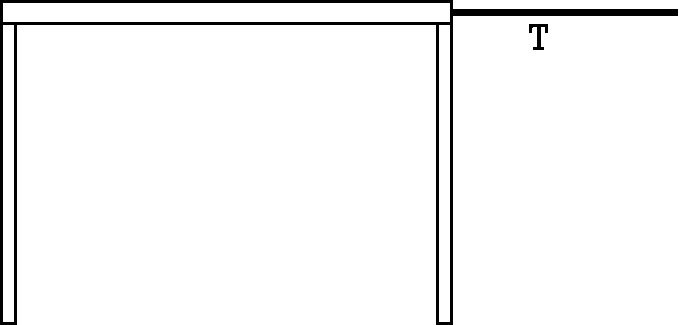
\includegraphics[width=0.7\textwidth]{table-crop.pdf}
%\end{center}
%\end{minipage}
%
%In this problem, you will calculate the required tension $T$ to tip the table.
%
%\begin{enumerate}
%
%\item Draw a force diagram for the table. Indicate your choice of pivot.
%
%\newpage
%
%\item What tension force $T$ is required to tip the table (so that the back legs come off the ground)?
%(Hint: What is true about the normal forces on the table when it begins to tip?)
%
%\vspace {4in}
%
%\item What coefficient of static friction between the legs and the floor is
%required so that the table tips, rather than sliding?
%
%\end{enumerate}
 \end{document}
